\chapter{Gruppen verwalten}\label{gruppenVerwalten}
\minitoc
\clearpage


\section{Gruppen verwalten}
\begin{figure}[ht]
	\centering
	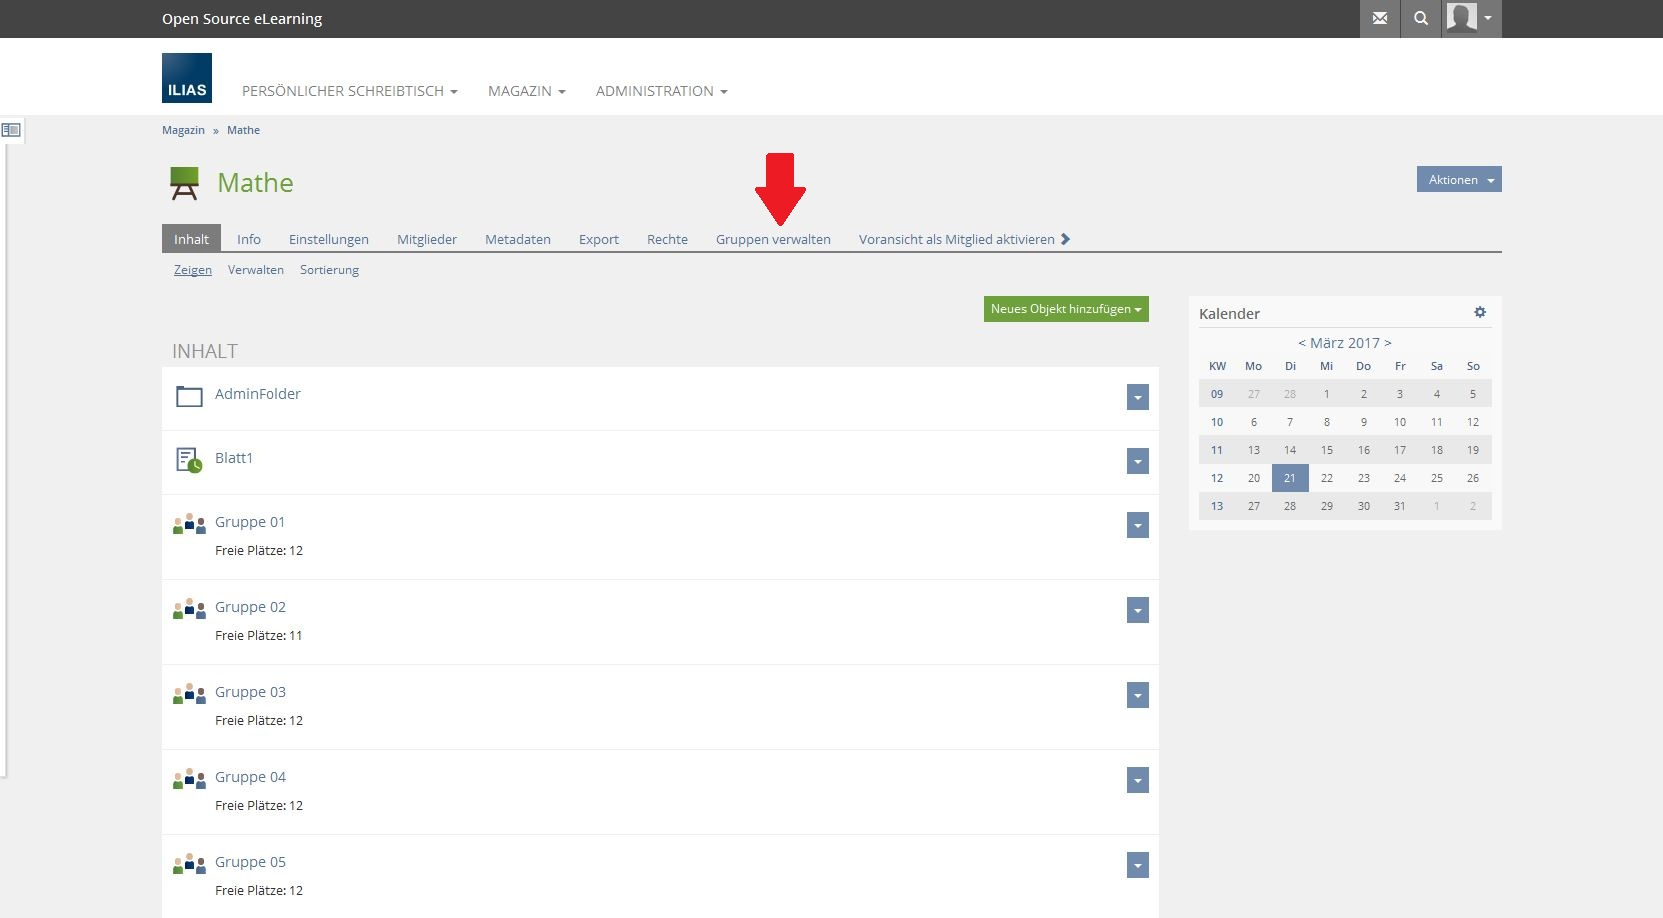
\includegraphics[width=1\textwidth]{img/gruppenverwalten.jpg}
	\caption{Ansicht Tab Gruppen verwalten im jeweiligen Kurs}
\end{figure}

~\\ In einem Kurs erscheint für alle Benutzer mit Schreibzugriff der neue Tab \textit{Gruppen verwalten}. In diesem Tab stehen drei Subtabs zur Auswahl. 
\begin{itemize}
	\item \textit{Gruppen erstellen} bietet die Funktionalität, mehrere Gruppen auf einmal zu erstellen. Dabei sind verschiedene Pflichtfelder und optionale Felder verfügbar.
	\item \textit{Kurs bearbeiten} bietet die Möglichkeit, Einstellungen mehrerer Gruppen auf einer Seite übersichtlich zu bearbeiten.
	\item \textit{Mitglieder verschieben} bietet die Möglichkeit, Mitglieder zwischen Gruppen hin- und herzuschieben. Voraussetzung dafür ist, dass der Benutzer bereits Mitglied in einer Gruppe ist. Um Tutoren zu verschieben, benutzen Sie bitte den Tab \textit{Kurs bearbeiten}. Tutoren bleiben der bisherigen Gruppe als Administrator erhalten, und werden der Ziel-Gruppe als Mitglied hinzugefügt.
\end{itemize} 
\clearpage


\section{Gruppen erstellen}
\begin{figure}[h!]
	\centering
	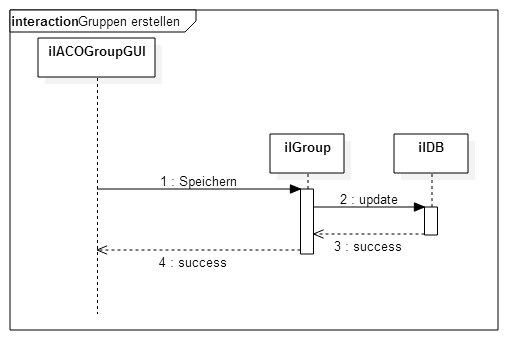
\includegraphics[width=.75\textwidth]{img/seq_groupGUI.png}
	\caption{Sequenzdiagramm Gruppen erstellen}
\end{figure}
\begin{figure}[h!]
	\centering
	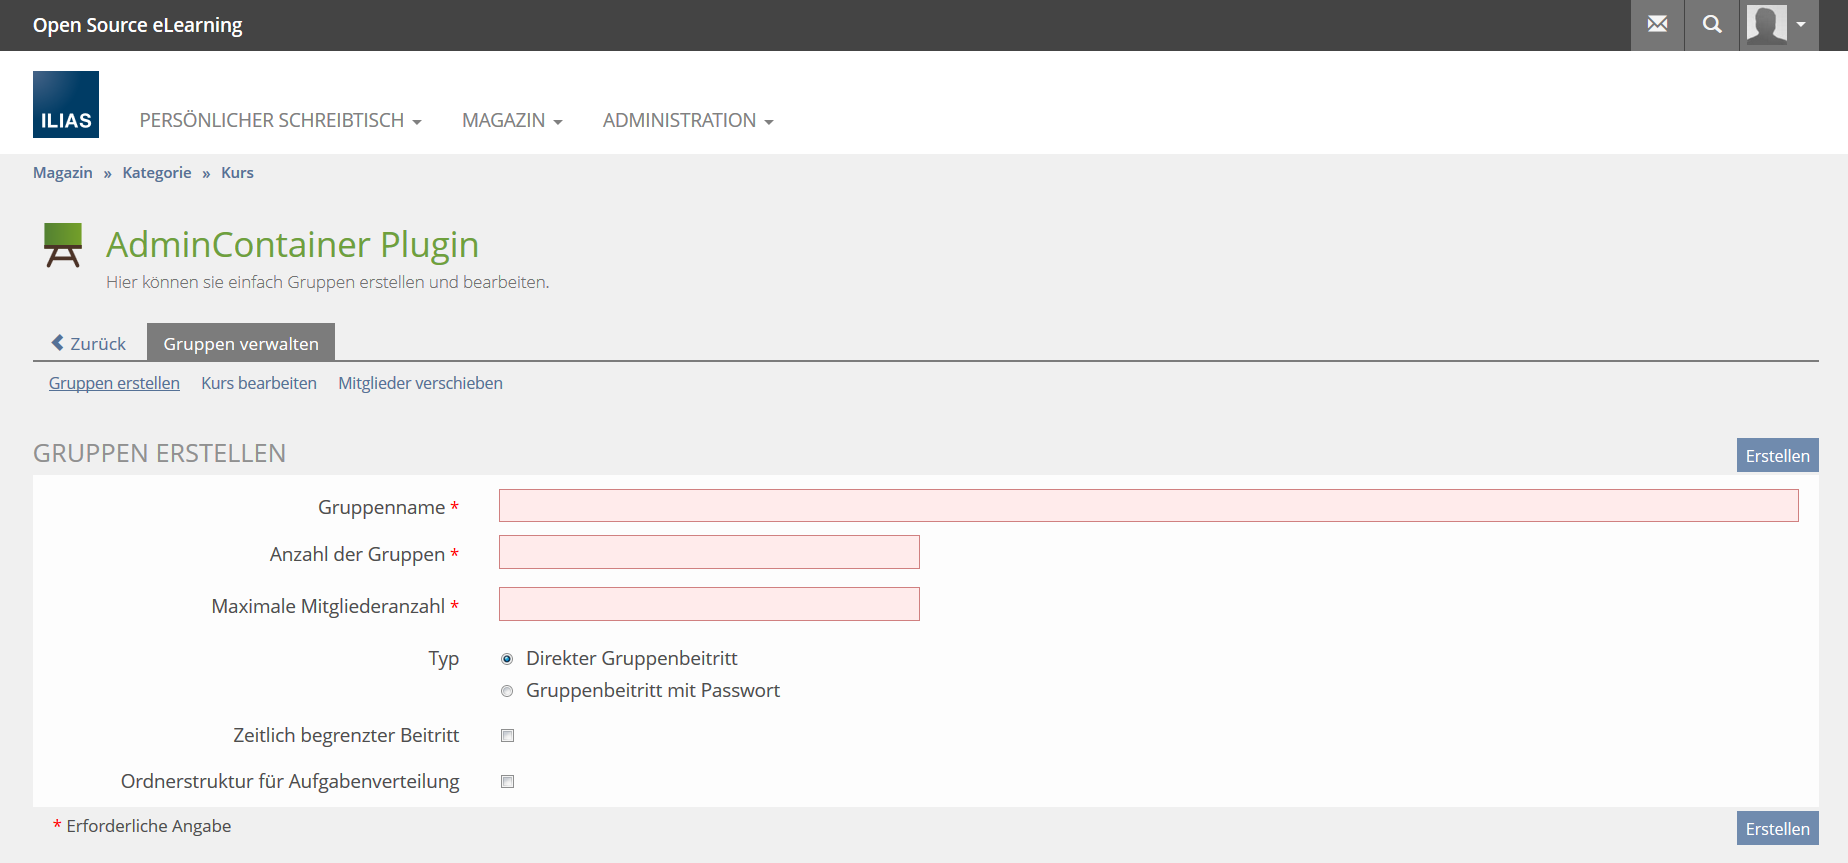
\includegraphics[width=1\textwidth]{img/gruppenErstellen.png}
	\caption{Ansicht Gruppen erstellen}
\end{figure}

In diesem Reiter/Tab lassen sich beliebig viele Gruppen erstellen. 
\newpage
\subsection*{Vorgehen - Pflichtfelder}

\begin{itemize}
	\item Eingeben eines Namenspräfix im Textfeld \textit{Gruppennamen} 
	\item Eingeben einer Zahl größer Null im Textfeld \textit{Anzahl der Gruppen}
	\item Eingeben einer Zahl im Textfeld \textit{Maximale Mitgliederanzahl} für die maximale Anzahl der Gruppenmitglieder 
\end{itemize}
(Versehentlich eingegebene Buchstaben werden bei Zahleneingaben ignoriert)




\subsection*{Vorgehen - optional}

\subsubsection*{Beitritts - Typ}
\begin{itemize}
	\item[1] Radiobutton auf  \textit{Gruppenbeitritt mit Passwort}   setzen, um die Gruppen mit einem Passwort zu schützen. 
	\item[2] Ein weiteres Textfeld taucht auf, bei dem das gewünschte Passwort einzugeben ist. (Passwort ist für alle Gruppen dasselbe)
\end{itemize}

\subsubsection*{Zeitlich begrenzter Beitritt}
\begin{itemize}
	\item[1] Checkbox setzen 
	\item[2] Zwei Datumseingabefelder tauchen für den Anmelde-Zeitraum auf, sowohl für Beitrittsanfang, als auch für Beitrittsende einen Zeitpunkt auswählen. Format: Tag / Monat / Jahr / Stunde / Minuten 
	(Achtung, Ende kann nicht vor Start liegen)
	
\end{itemize}

\subsubsection*{Ordnerstruktur für Aufgabenverteilung}
\begin{itemize}
	\item[1] Checkbox setzen 
	\item[2] Ein Textfeld taucht auf, bei dem man einen oder mehrere Ordnernamen (durch ";" getrennt) eingeben kann. Dadurch werden im Kurs, als auch in allen zu erstellenden Gruppen, diese Ordner mit den bzw. dem Namen erzeugt. Dies dient der vereinfachten Verteilung von Übungen bzw. Tests. (siehe auch \nameref{linkUebung} und \nameref{linkTest})
	
\end{itemize}
\clearpage

\section{Kurs bearbeiten}
\begin{figure}[h!]
	\centering
	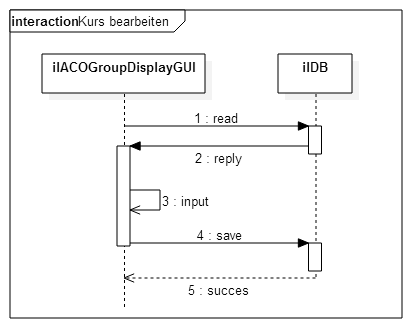
\includegraphics[width=.45\textwidth]{img/seq_groupdisplayGUI.png}
	\caption{Sequenzdiagramm Kurs bearbeiten}
\end{figure}
\begin{figure}[h!]
	\centering
	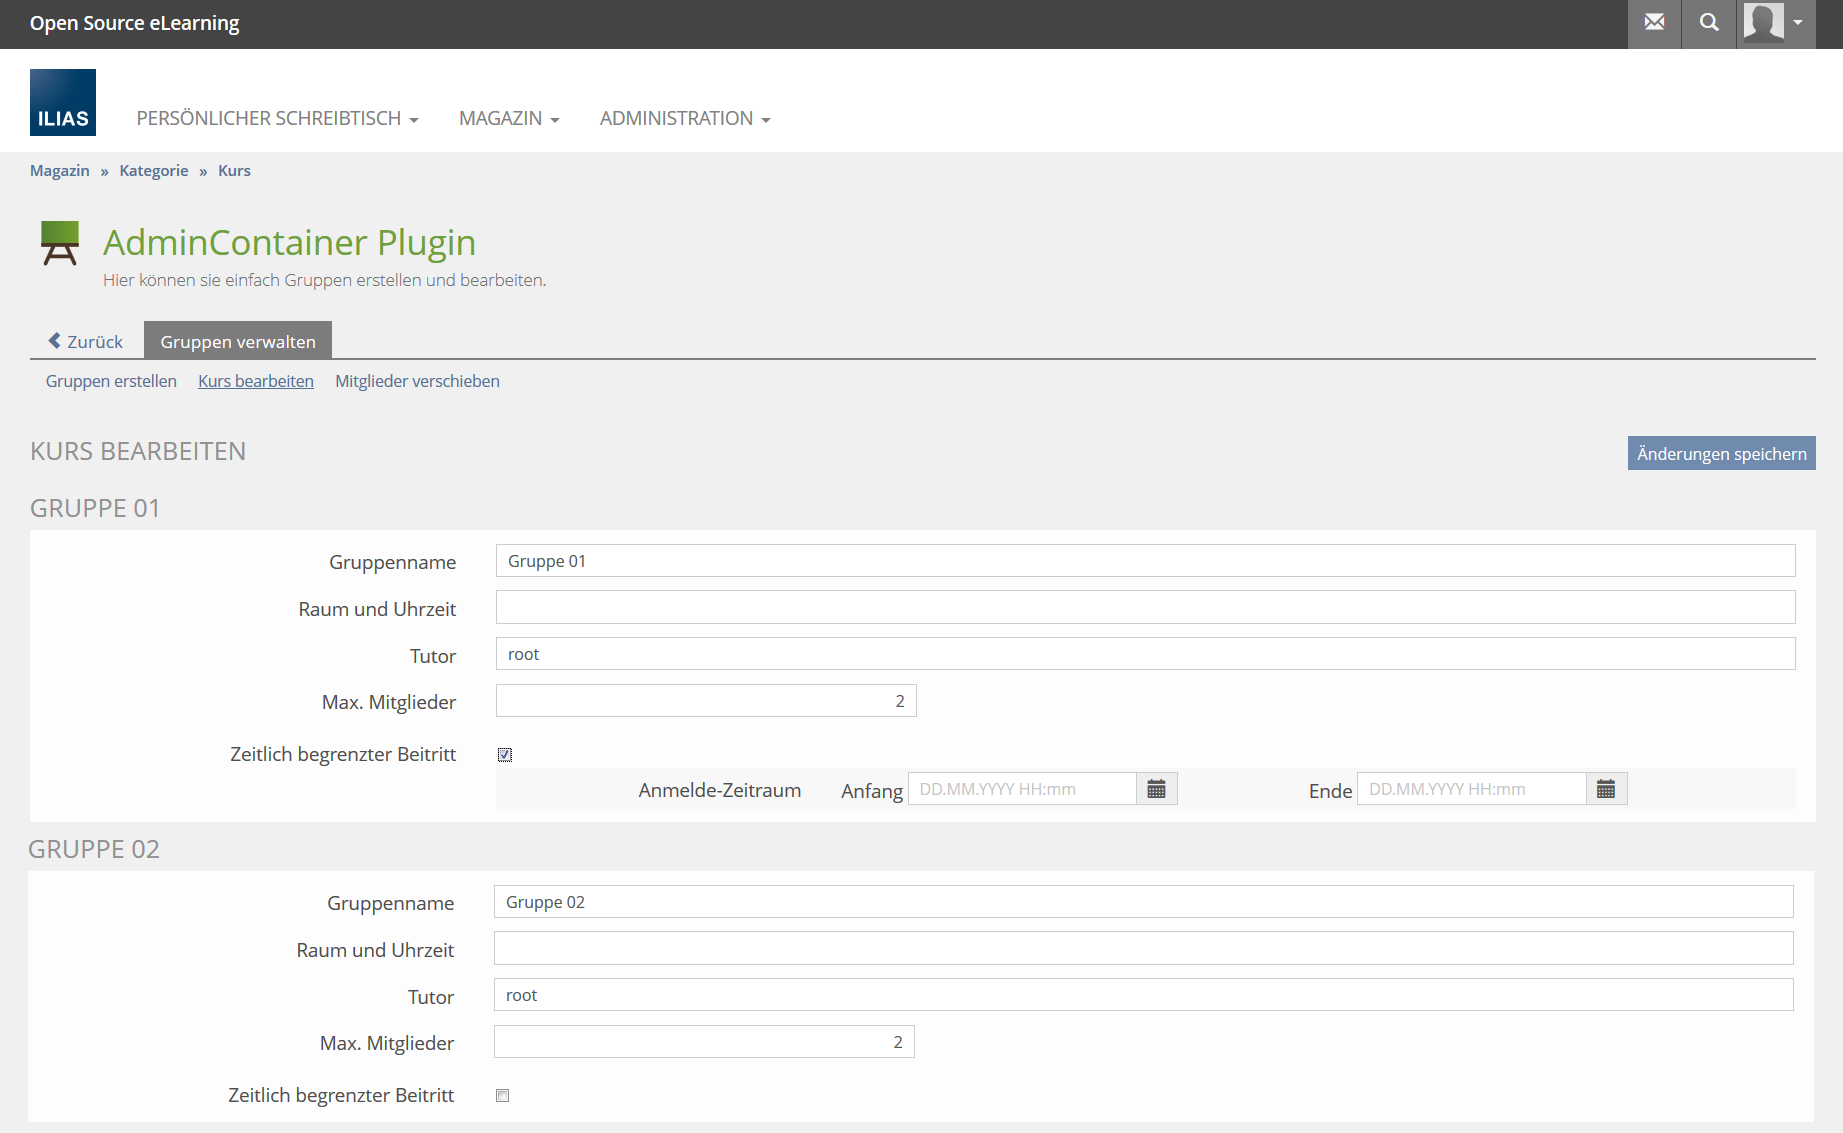
\includegraphics[width=.95\textwidth]{img/kursBearbeiten.png}
	\caption{Ansicht Kurs bearbeiten}
\end{figure}


~\\In diesem Reiter/Tab erhält man eine Übersicht aller im Kurs vorhandenen Gruppen mit folgenden Feldern.
\newpage
\subsection*{Gruppen}
Die Felder können einzeln und unabhängig voneinander bearbeitet werden. Felder zeigen den aktuellen Wert/Zustand der Gruppe an. 
Mit einem Klick auf den \textit{Änderung speichern} Knopf werden die Änderungen übernommen. 

\subsubsection{Gruppenname}
\begin{itemize}
	\item Auf das Feld klicken, um den Namen verändern, dies beinhaltet den Suffix, dessen Veränderung unter Umständen die Nummerierung durcheinander bringt. (Feld darf nicht leer sein)
\end{itemize}

\subsubsection{Raum und Uhrzeit - als Beschreibung}
\begin{itemize}
	\item In das Textfeld lässt sich eine beliebige Zeichenkette eintragen (z.B. Raum und Uhrzeit), die dann als Beschreibung der Gruppe auftaucht. 
\end{itemize}

\subsubsection{Tutor}
\begin{itemize}
	\item Um einem Benutzer die Tutor bzw. Gruppenadministrationsrechte zuzuweisen bzw. zu entziehen. 
	\item[hinzufügen] Um den Gruppenadministrator zu ändern, gibt man hier den Benutzernamen des neuen Administrators ein. Eine Auto-Complete Funktion hilft beim vervollständigen der Benutzernamen. Dem alten eingetragenen Benutzer werden damit die Adminrechte in der Gruppe entzogen, außer es handelt sich um einen Kursadministrator, dann wird der neue Administrator zusätzlich angelegt.
\end{itemize}

\subsubsection{Max Mitglieder}
Um den angezeigten Wert für die Gruppe zu verändern
\begin{itemize}
	\item Eingeben einer Zahl im Textfeld \textit{Maximale Mitgliederanzahl} für die maximale Anzahl der Gruppenmitglieder 
\end{itemize}


\subsubsection{Zeitlich begrenzter Beititt}
Wenn Checkbox nicht gesetzt, gibt es keinen zeitlich begrenzten Betritt bei dieser Gruppe. Um einen zu erzeugen
\begin{itemize}
\item[1] Checkbox setzen 
\item[2] Zwei Datumseingabefelder tauchen für den Anmelde-Zeitraum auf, sowohl für Beitrittsanfang, als auch für Beitrittsende einen Zeitpunkt auswählen. Format: Tag/Monat/Jahr/Stunde/Minuten 
(Achtung, Ende kann nicht vor Start liegen)
\end{itemize}

Ansonsten Checkbox deaktivieren und begrenzter Beitritt verschwindet. 
Falls schon ausgewählt und man nur das Datum verändern will, Schritt 1 überspringen. 


\clearpage

\section{Mitglieder verschieben}
\begin{figure}[h!]
	\centering
	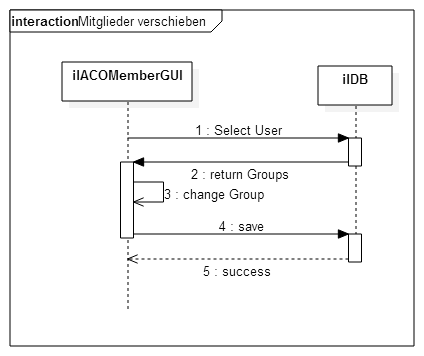
\includegraphics[width=.45\textwidth]{img/seq_memberGUI.png}
	\caption{Sequenzdiagramm Mitglieder verschieben}
\end{figure}

\begin{figure}[!ht]
	\centering
	\subfloat[Benutzer auswählen]{%
		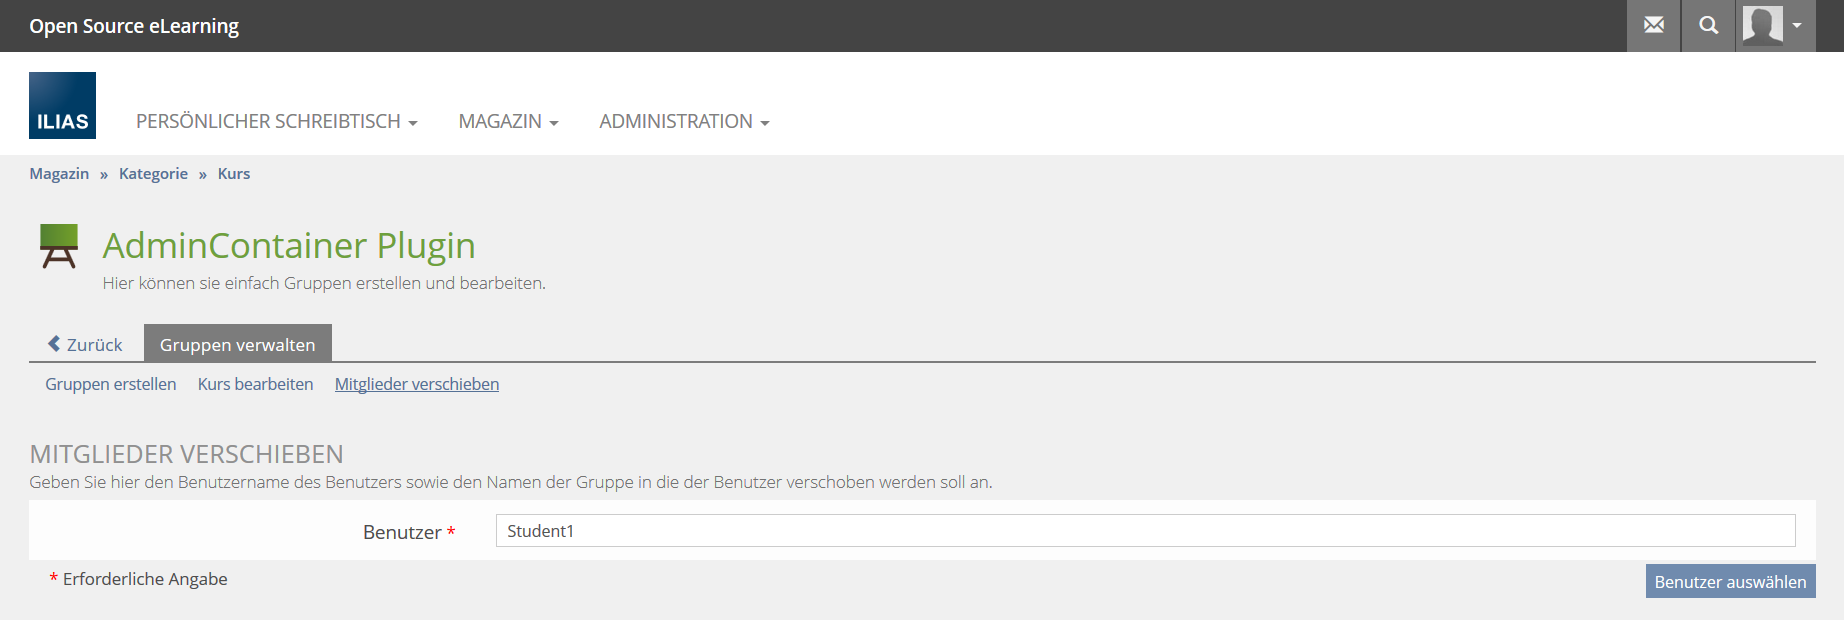
\includegraphics[width=0.93\textwidth]{img/mitgliederVerschieben1.png}
	}
	\hfill
	\subfloat[Gruppen auswählen]{%
		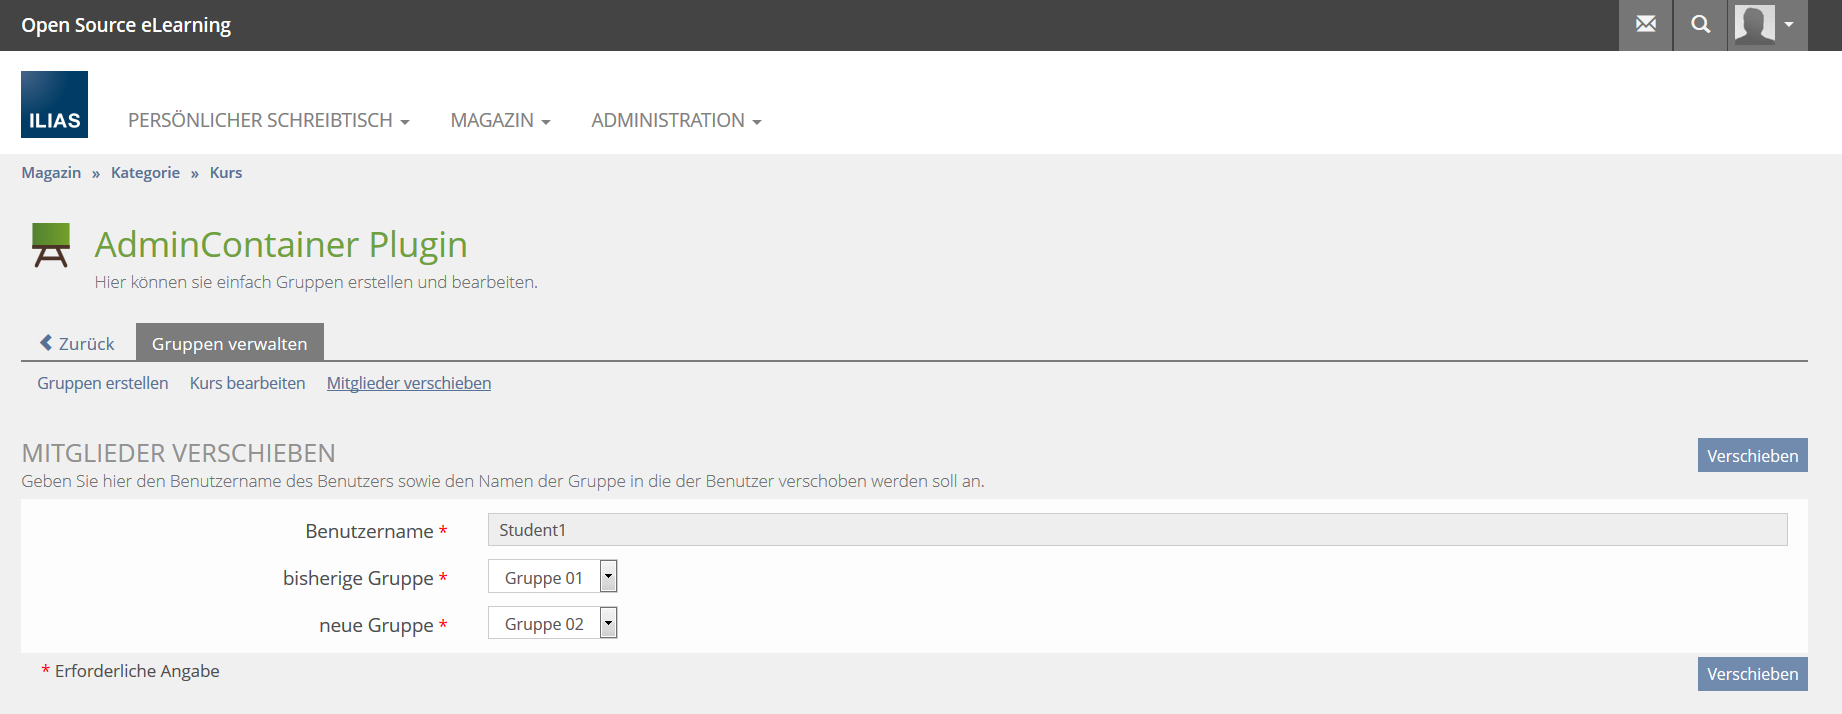
\includegraphics[width=0.93\textwidth]{img/mitgliederVerschieben2.png}
	}
	\caption{Ansicht Mitglieder verschieben}

\end{figure}

\newpage
\subsection*{Mitglieder verschieben}
\subsubsection*{Benutzer auswählen}
\begin{itemize}
	\item Benutzernamen eingeben, ab dem dritten Buchstaben hilft die Auto-Complete Funktion beim Vervollständigen. (Pflichtfeld, darf nicht leer sein)
	\item Auf \textit{Benutzer auswählen} klicken
\end{itemize}
\subsubsection*{Benutzer wurde ausgewählt}
\begin{itemize}
	\item Auf der neuen Seite wird in dem Drop-down Menü unter \textit{bisherige Gruppe} angezeigt, in welchen Gruppen sich der Benutzer befindet, darunter unter \textit{neue Gruppe}, die möglichen Gruppen zum verschieben.
	\item Auswählen, aus welcher Gruppe (Achtung im Drop-down von bisherige Gruppe Menü können mehrere Gruppen angezeigt werden, da sich Benutzer möglicherweise in mehreren Gruppen befindet) der Benutzer verschoben werden soll.
	\item Auswählen, in welche \textit{neue Gruppe} man den Benutzer verschieben will
	\item Mit dem Klicken auf \textit{Verschieben} die Eingabe bestätigen und den Benutzer verschieben
\end{itemize}


\clearpage